\begin{wrapfigure}[0]{r}[9pt]{0cm}
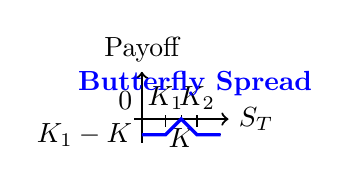
\begin{tikzpicture}[scale=1]
    % --- 定义坐标和参数 ---
    % 设定行权价，满足 K1 < K < K2。这里选取对称的值以便绘图美观。
    \def\Kone{0.3}       % 较低行权价 K1
    \def\K{0.5}          % 中间行权价 K
    \def\Ktwo{0.7}       % 较高行权价 K2
    % [用户要求] 设定 maxST
    \def\maxST{1.0}      % S_T 的最大显示范围

    % 计算两侧的负收益水平
    % 在对称情况下 (K - K1 = K2 - K)，这两个值相等。
    \def\wingPayoff{\Kone - \K} % S_T < K1 或 S_T > K2 时的收益 (例如 0.3 - 0.5 = -0.2)

    % --- 绘制坐标轴 ---
    % Y 轴 (Payoff) - 需要延伸到负值区域
    \draw[->, thick] (0, \wingPayoff - 0.1) -- (0, 0.6) node[above] {Payoff};
    % X 轴 (S_T)
    \draw[->, thick] (-0.1, 0) -- (\maxST + 0.1, 0) node[right] {$S_T$};

    % --- 绘制辅助线和标签 ---
    % 标记原点
    \node[above left] at (0, 0) {0};

    % 在 X 轴上标记 K1, K, K2
    \draw (\Kone, 0) node[above] {$K_1$} -- (\Kone, 0.05);
    \draw (\K, 0) node[below] {$K$} -- (\K, 0.05);
    \draw (\Ktwo, 0) node[above] {$K_2$} -- (\Ktwo, 0.05);

    % 在 Y 轴上标记负收益水平
    % 由于对称，K1-K 和 K-K2 是相等的水平
    \draw (0, \wingPayoff) node[left] {$K_1 - K$} -- (0.05, \wingPayoff);

    % 绘制辅助虚线
    % 水平线: 左侧从 Y 轴到 K1，右侧从 K2 到 maxST
    \draw[dashed, thin] (0, \wingPayoff) -- (\Kone, \wingPayoff);
    \draw[dashed, thin] (\Ktwo, \wingPayoff) -- (\maxST, \wingPayoff);
    % 垂直线: 从 K1 和 K2 向下到收益曲线
    \draw[dashed, thin] (\Kone, 0) -- (\Kone, \wingPayoff);
    \draw[dashed, thin] (\Ktwo, 0) -- (\Ktwo, \wingPayoff);
    % K 处的点在 (K, 0)，已经在轴上


    % --- 绘制 Butterfly Spread 收益曲线 (蓝色粗线) ---
    % 路径分析:
    % 1. S_T < K1: 恒定负收益 K1-K。从 (0, wingPayoff) 到 (K1, wingPayoff)。
    % 2. K1 <= S_T <= K: 收益线性上升到 0。从 (K1, wingPayoff) 到 (K, 0)。
    % 3. K <= S_T <= K2: 收益线性下降回到负值。从 (K, 0) 到 (K2, wingPayoff)。
    % 4. S_T > K2: 恒定负收益 K-K2 (等于 K1-K)。从 (K2, wingPayoff) 到 (maxST, wingPayoff)。
    \draw[blue, very thick] (0, \wingPayoff) -- (\Kone, \wingPayoff) -- (\K, 0) -- (\Ktwo, \wingPayoff) -- (\maxST, \wingPayoff);

    % --- 添加标题标签 ---
    % 将标题放在图像上方居中位置
    \node[blue, anchor=south, font=\bfseries, yshift=5pt, xshift=5pt] at (\K, 0) {Butterfly Spread};

\end{tikzpicture}
\end{wrapfigure}